There are many ways to skin a cat and there are many ways to plot data in Python. But using \link{https://matplotlib.org/}{matplotlib} is the obvious route and what we'll focus on. Matplotlib offers a major advantage of being integrated into pandas and being the most popular choice for anyone working with the broader Python community. \link{https://seaborn.pydata.org/}{Seaborn} is built on matplotlib and might be prettier out of the box. \link{https://plotnine.readthedocs.io/en/stable/}{Plotnine} is based off ggplot2, so it might be more comfortable turf for R users. 

While you're getting started, you'll likely be tempted to use MS Excel or Google Sheets instead of using matplotlib. Try to fight through. In the long-run, matplotlib will be more re-usable and provide more customization. 


Our reference for matplotlib is \cite{vanderplas2016python} Chapter 4. For another tutorial, check out \link{https://github.com/rougier/matplotlib-tutorial}{Nicolas Rougier's tutorial}. For book-length treatments, see \cite{rougier2021scientific} or \cite{clark2022story}. I have a few random tutorials on \link{https://www.youtube.com/channel/UC7zSpQsXo4ezksvHaGYTvzg}{my youtube channel}. 


There are two interfaces: a MATLAB-inspired interface and an object-oriented interface. That is, you can create plots with either of this code styles. First, we will work with the simpler MATLAB style. 

\section{MATLAB Interface}

The standard import and alias is as follows.

\begin{lstlisting}[language = Python]
import matplotlib.pyplot as plt
\end{lstlisting}

Here's a minimal working example for a plot.

\begin{lstlisting}
import numpy as np

x = np.linspace(0, 10, 100)
plt.plot(x, np.sin(x))
plt.plot(x, np.cos(x))

plt.show()
\end{lstlisting}

The \code{plot()} function makes a line plot. Using \code{plt.show()} is not always necessary in a Jupyter environment. See \link{https://jakevdp.github.io/PythonDataScienceHandbook/04.00-introduction-to-matplotlib.html}{VanderPlas Chapter 4} for a slightly more technical discussion. It's sufficient to think of \code{plt.show()} as ``finishing'' the plot. This can be helpful when you want to create multiple plots in one code block.

Compare the following two programs.

\begin{lstlisting}[language = Python]
x = np.linspace(0,10,100)

for i in range(0,10):
    
    y = np.ones(len(x)) * i
    plt.plot(x, y)
    plt.show()
\end{lstlisting}

\begin{lstlisting}[language = Python]
x = np.linspace(0,10,100)

for i in range(0,10):
    
    y = np.ones(len(x)) * i
    plt.plot(x, y)

plt.show()
\end{lstlisting}

The only difference is the indentation of \code{plt.show()} Observe the first creates ten different plots. The second creates just one plot. 


\subsection{Saving Figures}

You can use \code{plt.savefig} to save a plot. This must go before \code{plt.show()}. There are many supported filetypes. I am partial to png and pdf. A \code{dpi} argument can be used to set the image resolution. 

\begin{lstlisting}[language = Python]
x = np.linspace(0,10,100)

for i in range(0,10):
    
    y = np.ones(len(x)) * i
    plt.plot(x, y)

plt.savefig('example_figure.png', dpi = 300)
plt.show()
\end{lstlisting}


\subsection{Special Plots: Scatter, Histogram, and Bar Plots}

Scatter plots can be created with \code{plt.scatter()}. However, you can get some efficiency gain by instead using \code{plt.plot()} by specifying a marker, like \code{marker = 'O'}, and setting \code{linestyle = ''}. See \cite{vanderplas2016python} for further discussion. 

\medskip

\begin{tabular}{lr}
\toprule
Plot type &  Function  \\
\midrule
Scatter &  \code{plt.scatter(x,y, alpha = 0.1)} \\
Histogram &   \code{plt.hist(x, bins = 20)} \\
Bar Plot &  \code{plt.bar(x,y)} \\
Horizontal Bar Plot &  \code{plt.barh(x,y)} \\

\bottomrule
\end{tabular}

\subsection{Customizations}
There are many additional parameters for customization available in each of these plotting functions and methods. It would be a fool's errand to learn them all from the outset. Over time you will find yourself visiting matplotlib documentation and getting a sense of what's possible and what's not. 

You should be familiar with 

\medskip 

\begin{tabular}{lrr}
\toprule
Function, Method, or Keyword Parameter & What it does & Example Availability  \\
\midrule
\code{alpha} & set opacity & \code{plt.scatter()} \\
\code{figsize} & figure dimensions & \code{plt.subplots() plt.figure()} \\
\code{dpi} & figure resolution & \code{plt.savefig()} \\
\code{transparent} & transparent background & \code{plt.savefig()} \\
- & set aspect ratio & \code{ax.set_aspect()}  \\
- & vertical line & \code{ax.axvline} \code{plt.axvline()} \\
- & horizontal line & \code{ax.axhline} \code{plt.axhline()} \\
\bottomrule
\end{tabular}

\subsection{Pandas Integration}

There are Pandas methods that create Matplotlib objects. You'll get pretty far with \code{.plot()} and \code{.plot.bar()} or \code{.plot.barh()}. 

Let's return to our sleeplessness application. We can call \code{.plot.bar()} for a quick bar graph. 

\begin{lstlisting}[language = Python]
top_activities_before_sleeping = df1819[same & sleeping].prev_activity_name.value_counts(normalize = True).head()
top_activities_before_sleepless = df1819[same & sleepless].prev_activity_name.value_counts(normalize = True).head()

top_activities_before_sleeping.plot.bar()
\end{lstlisting}

These don't quite like in the first example where we could keep adding to a plot. For example, the below does not create a side-by-side barplot or even create accurate labels on the x-axis to account for the differing indices. 

\begin{lstlisting}[language = Python]
top_activities_before_sleeping = df1819[same & sleeping].prev_activity_name.value_counts(normalize = True).head()
top_activities_before_sleepless = df1819[same & sleepless].prev_activity_name.value_counts(normalize = True).head()

# This is bad!
top_activities_before_sleeping.plot.bar(color = 'red', alpha = 0.5)
top_activities_before_sleepless.plot.bar(color = 'blue', alpha = 0.5)
\end{lstlisting}

For a side-by-side plot, it is better to use a DataFrame instead of a Series. 

\begin{lstlisting}[language = Python]
a = pd.DataFrame(top_activities_before_sleeping)
a.columns = ['sleeping']

b = pd.DataFrame(top_activities_before_sleepless)
b.columns = ['sleepless']

a.join(b, how = 'inner').plot.bar()
\end{lstlisting}







\section{Object-oriented Interface}


\subsection{Introduction to the OO Interface}
\begin{center}
    \textit{This section is from \cite{clark2022story}.}
    
    \link{https://github.com/alexanderthclark/Matplotlib-for-Storytellers}{Github Link}
\end{center}


The object-oriented interface looks like this. 

\begin{lstlisting}[language = Python]
fig, ax = plt.figure(), plt.axes()
ax.plot(x,y)
ax.set_title("My Chart")
\end{lstlisting}

There is no such thing as a free lunch, so you will observe this interface requires more code to do the same exact thing. Its virtues will be more apparent later. Object-oriented programming (OOP) also requires some new vocabulary. OOP might be contrasted with procedural programming as another common method of programming. In procedural programming, the MATLAB-style interface being an example, the data and code are separate and the programmer creates procedures that operate on the program's data. OOP instead focuses on the creation of \emph{objects} which encapsulate both data and procedures. 

An object's data are called its \emph{attributes} and the procedures or functions are called \emph{methods}. In the previous code, we have figure and axes objects, making use of axes methods \code{plot()} and \code{set_title()}, both of which add data to the axes object in some sense, as we could extract the lines and title from \code{ax} with more code. Objects themselves are instances of a \emph{class}. So \code{ax} is an object and an instance of the Axes class. Classes can also branch into subclasses, meaning a particular kind of object might also belong to a more general class. A deeper knowledge is beyond our scope, but this establishes enough vocabulary for us to continue building an applied knowledge of matplotlib. Because \code{ax} contains its data, you can think of \code{set_title()} as changing \code{ax} and this helps make sense of the \code{get_title()} method, which simply returns the title belonging to \code{ax}. Having some understanding that these objects contain both procedures and data will be helpful in starting to make sense of intimidating programs or inscrutable documentation you might come across.  %These are Just as there is a \code{set_title()}

\subsubsection{Figure, Axes}

A plot requires a figure object and an axes object, typically defined as \code{fig} and \code{ax}. The figure object is the top level container. In many cases like in the above, you'll define it at the beginning of your code and never need to reference it again, as plotting is usually done with axes methods. A commonly used figure parameter is \code{figsize}, to which you can pass a sequence to alter the size of the figure. Both the figure and axes objects have a \code{facecolor} parameter which might help to illustrate the difference between the axes and figure. 

\begin{lstlisting}[language = Python, caption = {[figparams.py]}]
fig = plt.figure(figsize = (2,3), 
                 facecolor = 'gray') 
ax = plt.axes(facecolor = 'lightyellow')
\end{lstlisting}

\begin{center}
    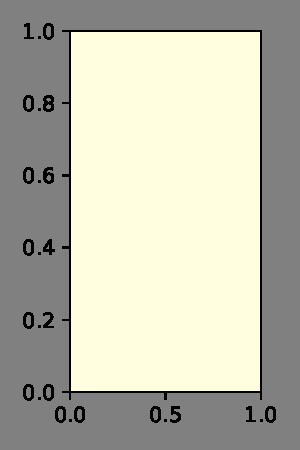
\includegraphics[width = .45\textwidth]{proseplots/figparams.pdf}
\end{center}


The axes object, named \code{ax} by convention, gets more use in most programs. In place of \code{plt.plot()}, you'll use \code{ax.plot()}. Similary, \code{plt.hist()} is replaced with \code{ax.hist()} to create a histogram. If you have experience with the MATLAB interface, you might get reasonably far with the object-oriented style just replacing the \code{plt} prefix on your pyplot functions with \code{ax} to see if you have an equivalent axes method.

This wishful coding won't take you everywhere though. For example, \code{plt.xlim()} is replaced by \code{ax.set_xlim()} to set the $x$-axis view limits. To modfiy the title, \code{plt.title()} is replaced with \code{ax.set_title()} and there is \code{ax.get_title()} simply to get the title. The axes object also happens to have a \code{title} attribute, which is only used to access the title, similar to the \code{get_title()} method. Many matplotlib methods can be classified as \emph{getters} or \emph{setters} like for these title methods. The plot method and its logic is different. Later calls of \code{ax.plot()} don't overwrite earlier calls and there is not the same getter and setter form. There's a \code{plot()} method but no single \code{plot} attribute being mutated. Whatever has been plotted can be retrieved, or gotten (getter'd?), but it's more complicated and rarely necessary. Use the code below to see what happens with two calls of \code{plot()} and two calls of \code{set_title()}. The second print statement demonstrates that the second call of \code{set_title()} overwrites the title attribute, but a second plot does not nullify the first. 

%It's part of the object-oriented construction, which goes beyond our scope.
%\newpage

 
\begin{lstlisting}[language = Python, caption= {[gettersetter.py]}]
x = np.linspace(0,1,2)    (*@\margintext{gettersetter}@*) 
fig, ax = plt.figure(figsize = (8,4)), plt.axes()
ax.plot(x, x)
ax.plot(x, 1 - x)
ax.set_title("My Chart")
print(ax.title)
print(ax.get_title()) # Similar to above line
ax.set_title("My Wholesome Chart")
print(ax.get_title()) # long
\end{lstlisting}

\begin{center}
    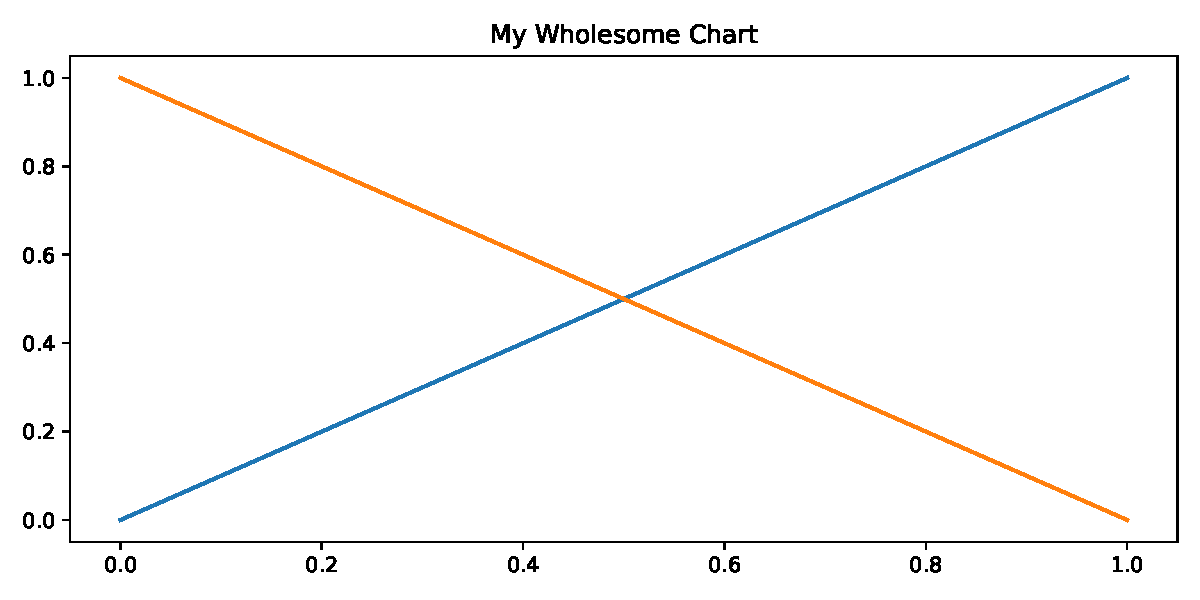
\includegraphics[width = .7\textwidth]{proseplots/gettersetter.pdf}
\end{center}

Axes methods \code{set_xlim()} and \code{get_xlim()} behave just like \code{set_title()} and \code{get_title()}, but note there is no attribute simply accessible with \code{ax.xlim}, so the existence of getters and setters is the more fundamental pattern.\footnote{Getters and setters are thought of as old-fashioned. It's more Pythonic to access attributes directly, but matplotlib doesn't yet support this.}
%https://matplotlib.org/stable/tutorials/intermediate/artists.html?highlight=artist%20tutorial for old fashioned comment

\subsubsection{Mixing the Interfaces}

You can also mix the interfaces. Use \code{plt.gca()} to \emph{g}et the \emph{c}urrent \emph{a}xis. Use \code{plt.gcf()} to \emph{g}et the \emph{c}urrent \emph{f}igure.

\begin{lstlisting}[language = Python, caption={[chart.py]}]
x = np.linspace(0,1,2) 
plt.plot(x,x)
plt.title("My Chart")

ax = plt.gca()
print(ax.title)

ax.plot(x, 1 - x)
ax.set_title('My Wholesome Chart')
print(ax.title)

fig = plt.gcf()
fig.savefig('chart.pdf') # same as plt.savefig
\end{lstlisting}

\begin{center}
    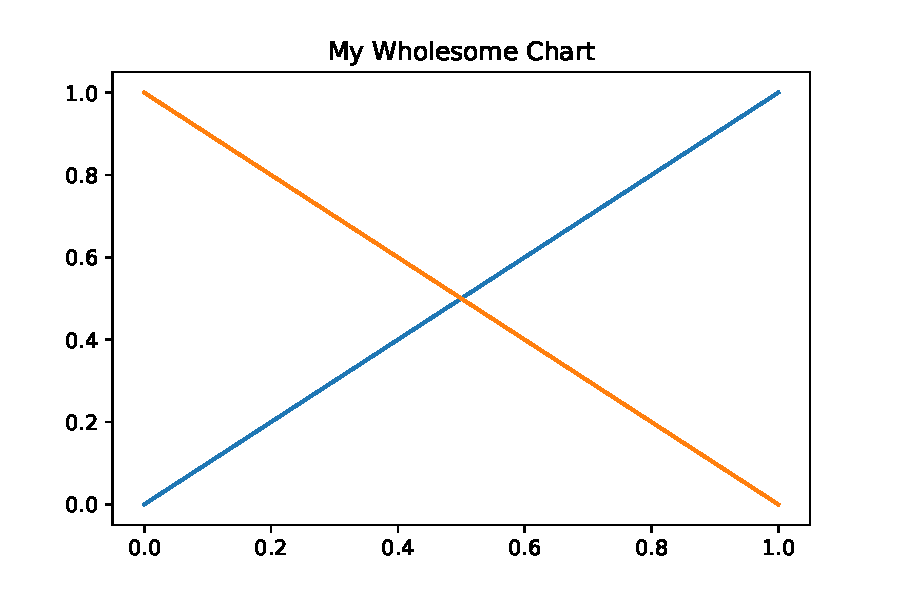
\includegraphics[width = .8\textwidth]{proseplots/chart.pdf}
\end{center}


In the above, we started with MATLAB and then converted to object-oriented. We can also go in the opposite direction as well. We can also mix pandas with MATLAB or OOP-style matplotlib. 

These plots can be mixed with the object-oriented interface. You can use a plot method and specify the appropriate axes object as an argument. Below we import the iris dataset and make a boxplot with a mix of axes methods and then pyplot functions. 

\begin{lstlisting}[language = Python, caption= {[irisbox.py]}]
from sklearn.datasets import load_iris 
data = load_iris()['data']
df = pd.DataFrame(data)

fig, ax = plt.figure(), plt.axes()

df.plot.box(ax = ax)
ax.yaxis.grid(True)
ax.xaxis.grid(False)

plt.tight_layout()
plt.savefig('irisbox.pdf')
\end{lstlisting}

\begin{center}
    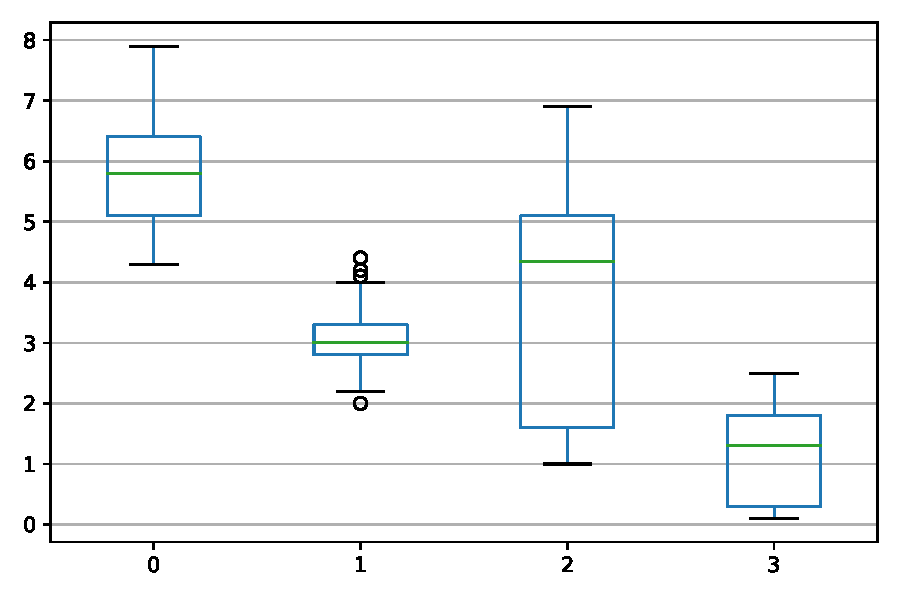
\includegraphics[width = .7\textwidth]{proseplots/irisbox.pdf}
\end{center}



\subsection{Subplots with \code{plt.subplots()}}

You can use \code{subplots()} to create multiple subplots within the figure.

\begin{lstlisting}[language = Python]
# Multiple Subplots
# ax is a tuple for two different axes
fig, ax = plt.subplots(1,2)

# Call plot() on the axis
ax[0].plot(x, np.sin(x))
ax[1].plot(x, np.sin(x), color = 'tomato')

plt.show()
\end{lstlisting}

In the last example above, two subplots are created. If you save this, note this creates a single image file, not one for each subplot. Next, we create a $2\times 2$ grid. Note, when we do this, we must index \code{ax} at two layers. Before, in a $1\times2$, we had one-dimensional indexing. The superfluous second dimension was \emph{squeezed} out by default.\footnote{See the \code{squeeze} parameter in the \link{https://matplotlib.org/3.5.0/api/_as_gen/matplotlib.pyplot.subplots.html}{documentation}.}

\begin{lstlisting}[language = Python]
fig, ax = plt.subplots(2,2)

x = np.linspace(0, 2 * np.pi)
y = np.sin(x)

ax[0,0].plot(x,y)
ax[0,1].plot(x,y, linestyle = 'dashed')
ax[1,0].plot(x,y, linestyle = 'dotted', color = 'black')
ax[1,1].plot(x,y, linewidth = 7)

for ax_ in fig.axes:
    ax_.set_title('Sine Wave')

fig.suptitle("Big Plot", size = 20)
plt.tight_layout()

plt.savefig("subplot_example_2by2.pdf")
\end{lstlisting}

\begin{center}
    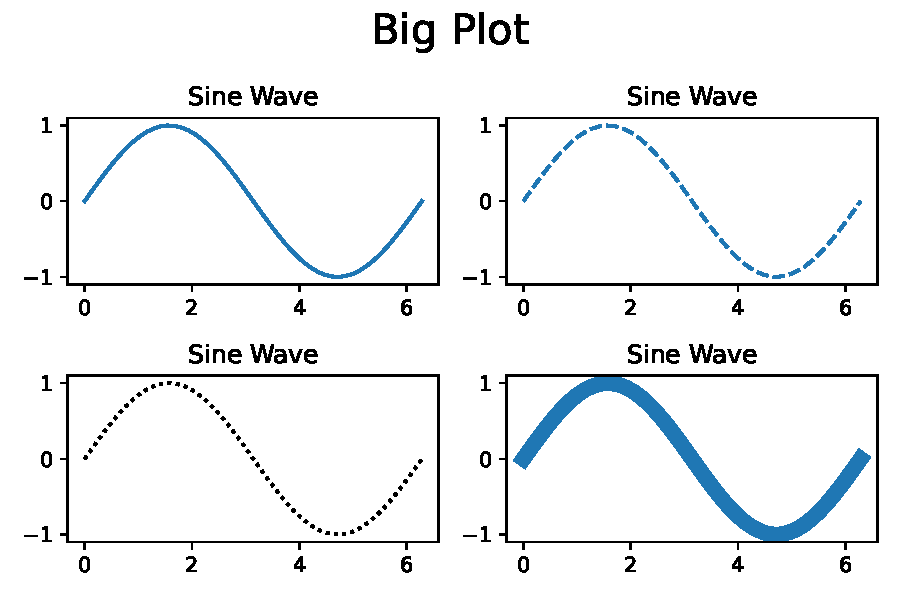
\includegraphics[width = .6\textwidth]{images/subplot_example_2by2.pdf}
\end{center}